\chapter{Appendix}\label{chap:appendix}
\section{Model Fitting}\label{sec:modelfitting}
The model fitting was carried out with \textit{SciPy} and \textit{NumPy} in the python programming language. In the case of the exponential model fit \textit{SciPy} provides a optimizer \textit{scipy.optimizer}, which provides the \textbf{curve\_fit} method \cite{SciPyCurveFit}. This method uses the Levenberg-Marquardt method to solve non-linear least squared problems. \textit{NumPy} delivers the \textbf{polyfit} method, which was used to fit the MSE data to the polynomial model described in equation \ref{eq:polyfit}. The linear regression is achieved using \textit{scipy.stats} \textbf{linregress} method, which calculates a linear least-squares regression for two sets of data points for x and y \cite{SciPyLinRegress}.

\subsection{Levenberg-Marquardt Method}\label{subsec:lmMethod}
The Levenberg-Marquardt method is a hybrid of the Gauss-Newton method and the Levenberg-method (Trust-Region approach). Starting from an initial guess for the parameters, the Levenberg-Marquardt method uses the Jacobian matrix to estimate how changes in parameters affect the fitted function. Then a damped least squared step is applied, where if the parameters are far from optimal, the Levenberg-Marquardt method behaves like the gradient descent, and if the parameters are near optimal the Levenberg-Marquardt method acts like the Gauss-Newton method. It minimizes the sum of the squared residuals:
\begin{align}
    f(x)=\frac{1}{2}\sum_{j=1}^{m}{r_{j}^{2}(x)=\frac{1}{2}||r||^{2}},
\end{align}
where $f(x)$ is the objective function that we are trying to minimize, $r_{j}(x)$ represent the residuals (which are the differences between the observed data and the model predictions), $r(x)$ is the vector of residuals, where $r(x)=[r_{1}(x), r_{2}(x),...,r_{n}(x)]^T$. $||r||^{2}$ is the squared Euclidean norm of the residual vector, which sums the squared differences. The Gauss-Newton method is modified by a damping coefficient $\lambda$ and is written as:
\begin{align}
    (J^{T}J+ \lambda I)p = J^{T}r(x),
\end{align}
where J is the Jacobian matrix of $r(x)$ (the derivatives of the residuals), $I$ is the identity matrix and $\lambda$ controls the step size (a large $\lambda$ leads to gradient descent, small $\lambda$ lead to the Gauss-Newton method). $J^{T}J$ is the approximation of the Hessian matrix. $p$ is the update step. This equation is solved iteratively reducing $f(x)$ until the parameters converge.

If $\lambda$ is large, the equation behaves like the gradient descent:
\begin{align}
    \lambda I p= J^{T}r(x),
\end{align}
while a small $\lambda$ causes the equation to behave like the Gauss-Newton method:
\begin{align}
    J^{T}Jp=J^{T}r(x).
\end{align}
\cite{gavin2020levenberg} \cite{Levenberg-Marquardt} \cite{broxOptimierung}

\subsection{Linear Regression by SciPy}\label{subsec:linreg}
SciPy's \textbf{linregress} method fits data to a simple linear model as depicted in equation \ref{eq:linreg}. It achieves this by solving the \textit{Ordinary Least Squares} regression which minimizes the sum of squared residuals. It returns the slope and the intercept of the fitted line, as well as the \textit{R-value} (\textit{Pearson's R}), \textit{p-value}, standard error  of the estimated slope and the standard error of the estimated intercept.
\cite{SciPyLinRegress} \cite{Wooditch2021}

\subsection{polyfit and polyval by Numpy}\label{subsec:polyfit}
The \textit{numpy.polyfit} method fits a polynomial of a given degree to a set of data points using the least squares minimization method \cite{NumPyPolyfit}. This method constructs the Vandermonde Matrix of a degree $d$ and a set of data points $(x_{1}, y_{1}), (x_{2}, y_{2}), ...,(x_{n}, y_{n})$ of form:
\begin{align}
    V =
    \begin{bmatrix} 
        x_{1}^{d} & x_{1}^{d-1} & \dots & x_{1}^{1} & 1 \\
        x_{2}^{d} & x_{2}^{d-1} & \dots & x_{2}^{1} & 1 \\
        \vdots & \vdots & \ddots & \vdots & \vdots \\
        x_{n}^{d} & x_{n}^{d-1} & \dots & x_{n}^{1} & 1 \\ 
    \end{bmatrix}
\end{align}
Each row represents one data point, and each column corresponds to a power of $x$. Following the construction of the Vandermonde-matrix, the polynomial coefficients $c=[c_{d},c_{d-1},...,c_{0}]$ are computed by solving:
\begin{align}
    c=(V^{T}V)^{-1}V^{T}y.
\end{align}
This method solves the linear least squares and ensures that the sum of squared residuals is minimized:
\begin{align}
    \sum_{i=1}{(y_{i}-P(x_i))^{2}}^{n},
\end{align}
where $P(x_i)$ is the polynomial function. \cite{NumPyPolyfit} \cite{Vandermonde} \cite{GATechLS}

Once the polynomial coefficients are computed, the polynomial is evaluated using numpy's \textbf{polyval} method. This method internally uses the \textit{Horner's method} in order to reduce the number of multiplications. For the polynomial of form:
\begin{align}
    P(x) = a_{n}x^{n}+a_{n-1}x^{n-1}+ \dots + a_{1}x+a_{0}
\end{align}
this method outputs a polynomial of form:
\begin{align}
    P(x)=p_{0}x^{n}+p_{1}^{n-1}+\dots + p_{n}.
\end{align}
\cite{wolfram_horner}

\section{Overview of Simulation Outcomes}\label{sec:overviewSimOutcomes}
The simulation outcomes are presented in the tables \ref{table:overviewcompletegraph}, \ref{table:overviewstar}, \ref{table:overviewring}, \ref{table:overviewtorus}, \ref{table:overview_Lollipop512_512}, \ref{table:overview_L128_896} \ref{table:overview_L896_128}, \ref{table:overview_ROC_32_32}, \ref{table:overview_ROC_128_8} and \ref{table:overview_ROC_8_128}. The tables contain the equations for the fitted models, the slopes in all regions and the MSE value after 100 rounds of execution of the algorithms.

\begin{sidewaystable}
  \centering
  \caption{Simulation Overview - Complete graph: Fitted Model, Slopes per Region, and Final MSE}
  \label{table:overviewcompletegraph}
  \begin{tabular}{ll l c c c c c}
      \toprule
      \multicolumn{2}{l}{\textbf{Topology}} & \textbf{Fitted Model} & \textbf{Slope (log-linear)} \\ 
      & & & \shortstack{Rounds \\ 1--10} & \shortstack{Rounds \\ 11--65} & \shortstack{Rounds \\ 66--100} & \shortstack{Rounds \\ 1--100} & \shortstack{$MSE_{100}$} \\
      \midrule
      \multirow{3}{*}{$K_{1024}$} 
      & DAB   & \shortstack{\textbf{Rounds 1--100:} \\ $MSE_r = 844.63 \cdot e^{-0.01r}$}   & $-2.6 \times 10^{-3}$  & $-2.7 \times 10^{-3}$  & $-3.0 \times 10^{-3}$  & $-2.8 \times 10^{-3}$   & 436.85 \\
      & PPS   & \shortstack{\textbf{Rounds 10--80:} \\ $MSE_r = 2530.41 \cdot e^{-0.9r}$} & -0.38   & -0.39 & -0.16  & -0.31  & $1.73\times10^{-28}$ \\
      & ATPPS & \shortstack{\textbf{Rounds 10--65:} \\ $MSE_r = 4309.94 \cdot e^{-1.06r}$}   & -0.43   & -0.46 & -0.02  & -8.4  & $5.63\times10^{-28}$ \\
      \bottomrule
  \end{tabular}
\end{sidewaystable}


\begin{sidewaystable}
    \centering
    \caption{Simulation overview - Star graph: fitted model, slopes per region, and final MSE}
    \label{table:overviewstar}
    \begin{tabular}{ll l c c c c c}
        \toprule
        \multicolumn{2}{l}{\textbf{Topology}} & \textbf{Fitted Model} & \textbf{Slope (log-linear)} \\ 
        & & & \shortstack{Rounds \\ 1--10} & \shortstack{Rounds \\ 11--45} & \shortstack{Rounds \\ 46--100} & \shortstack{Rounds \\ 1--100} & \shortstack{$MSE_{100}$} \\
        \midrule
        \multirow{3}{*}{$S_{1024}$} 
        & DAB   & \shortstack{\textbf{Rounds 1--100:} \\ $MSE_r = 840.42 \cdot e^{-0.01r}$} & $-2.3 \times 10^{-3}$ & $-2.3 \times 10^{-3}$ & $-2.5 \times 10^{-3}$ & $-2.4 \times 10^{-3}$ & 480.48 \\
        & PPS   & \shortstack{\textbf{Rounds 10--45:} \\ $MSE_r = 29794.60 \cdot e^{-1.39r}$} & -0.5  & -0.6 & $-4.8 \times 10^{-3}$ & -0.26 & $8.31 \times 10^{-25}$ \\
        & ATPPS & \shortstack{\textbf{Rounds 18--60:} \\ $MSE_r = 9329.40 \cdot e^{-1.05r}$} & -0.45  & -0.45 & -0.11 & -0.26 & $6.52 \times 10^{-24}$ \\
        \bottomrule
    \end{tabular}
  \end{sidewaystable}
  

\begin{sidewaystable}
    \centering
    \caption{Simulation overview - Ring graph: fitted model, slopes per region, and final MSE}
    \label{table:overviewring}
    \begin{tabular}{ll l c c c c c}
        \toprule
        \multicolumn{2}{l}{\textbf{Topology}} & \textbf{Fitted Model} & \textbf{Slope (log-log)} \\ 
        & & & \shortstack{Rounds \\ 1--10} & \shortstack{Rounds \\ 11--69} & \shortstack{Rounds \\ 70--100} & \shortstack{Rounds \\ 1--100} & \shortstack{$MSE_{100}$} \\
        \midrule
        \multirow{3}{*}{$R_{1024}$} 
        & DAB   & \shortstack{\textbf{Rounds 10--60:} \\ $MSE_r=1.72 \times 10^{-5}r^{4} - 2.30 \times 10^{-3}r^{3}$\\ 
        $ + 0.19r^{2} - 5.99r + 114.83$} & -1.1 & -0.51 & -0.5 & -0.78  & 22.41 \\
        & PPS   & \shortstack{\textbf{Rounds 10--60:} \\ $MSE_r= 2.99 \times 10^{-5}r^{4} - 0.5 \times 10^{-2}r^{3}$ \\ $+ 0.32r^{2} - 9.68r + 166.30$} & -0.93 & -0.55 & -0.52 & -0.74  & 27.68 \\
        & ATPPS & \shortstack{\textbf{Rounds 10--60:} \\ $MSE_r= 3.04 \times 10^{-5}r^{4} - 0.5 \times 10^{-2}r^{3}$ \\ $+ 0.32r^{2} - 9.64r + 161.86$} & -0.95 & -0.56 & -0.49 & -0.75  & 26.56 \\
        \bottomrule
    \end{tabular}
  \end{sidewaystable}
  

\begin{sidewaystable}
  \centering
  \caption{Simulation overview - Torus Grid: fitted model, slopes per region, and final MSE}
  \label{table:overviewtorus}
  \begin{tabular}{ll l c c c c c}
      \toprule
      \multicolumn{2}{l}{\textbf{Topology}} & \textbf{Fitted Model} & \textbf{Slope} \\ 
      & & & \shortstack{Rounds \\ 1--10} & \shortstack{Rounds \\ 10--39} & \shortstack{Rounds \\ 40--100} & \shortstack{Rounds \\ 1--100} & \shortstack{$MSE_{100}$} \\
      \midrule
      \multirow{3}{*}{$T_{32,32}$} 
      & DAB   & \shortstack{\textbf{Rounds 10--39:} \\ 
      $MSE_r = -1.35 \times 10^{-6}r^{5} + 1.89 \times 10^{-4}r^{4}$ \\ 
      $- 0.01r^{3} + 0.30r^{2} - 4.6r + 34.10$ \\ 
      \textbf{Rounds 40--100:} \\ 
      $MSE_r = -6.01 \times 10^{-6}r^{3} + 1.66 \times 10^{-3}r^{2}$ \\ 
      $- 0.16r + 6$} 
      & -2.1 & -1.2 & -2 & -1.7 & 436.85 \\
      
      & PPS   & \shortstack{\textbf{Rounds 10--39:} \\ 
      $MSE_r = -3.65 \times 10^{-6}r^{5} + 5.16 \times 10^{-4}r^{4}$ \\ 
      $- 0.03r^{3} + 0.83r^{2} - 12.52r + 88.16$ \\ 
      \textbf{Rounds 40--100:} \\ 
      $MSE_r = -1.15 \times 10^{-5}r^{3} + 3.205 \times 10^{-3}r^{2}$ \\ 
      $- 0.33r + 13.72$} 
      & -1.5 & -1.2 & -1.4 & -1.4 & $1.73 \times 10^{-28}$ \\

      & ATPPS & \shortstack{\textbf{Rounds 10--39:} \\ 
      $MSE_r = -5.54 \times 10^{-6}r^{5} + 7.65 \times 10^{-4}r^{4}$ \\ 
      $- 0.04r^{3} + 1.16r^{2} - 16.81r + 112.86$ \\ 
      \textbf{Rounds 40--100:} \\ 
      $MSE_r = -9.99 \times 10^{-6}r^{3} + 2.8034 \times 10^{-3}r^{2}$ \\ 
      $- 0.28r + 11.29$} 
      & -1.6 & -1.3 & -1.7 & -1.5 & $5.63 \times 10^{-28}$ \\
      \bottomrule
  \end{tabular}
\end{sidewaystable}


\begin{sidewaystable}
  \centering
  \caption{Simulation overview for $L_{512,512}$: fitted model, slopes per region, and final MSE}
  \label{table:overview_L512_512}
  \begin{tabular}{ll l c c c c c}
      \toprule
      \multicolumn{2}{l}{\textbf{Topology}} & \textbf{Fitted Model} & \textbf{Slope} \\ 
      & & & \shortstack{Rounds \\ 1--7} & \shortstack{Rounds \\ 8--50} & \shortstack{Rounds \\ 51--100} & \shortstack{Rounds \\ 1--100} & \shortstack{$MSE_{100}$} \\
      \midrule
      \multirow{3}{*}{$L_{512,512}$} 
      & DAB   & \makecell[l]{$MSE_r=-5.89\times10^{-5}r^{3}+0.03r^{2}$ \\ $-5.68r+459.42$} & -67 & -4.5 & -2.6 & -7.3 & 108.90 \\
      & PPS   & \makecell[l]{$MSE_r=8.44\times 10^{-7}r^{4}-2.52\times 10^{-4}r^{3}$ \\ $-0.03r^{2}-1.64r+56.68$} & -130 & -0.9 & -0.12 & -8.3 & 14.71 \\
      & ATPPS & \makecell[l]{$MSE_r=8.69 \times 10^{-7}r^{4}-2.56 \times 10^{-4}r^{3}$ \\ $+0.03r^{2}-1.62r+54.48$} & -130 & -0.87 & -0.12 & -8.3 & 13.82 \\
      \bottomrule
  \end{tabular}
\end{sidewaystable}

\begin{sidewaystable}
  \centering
  \caption{Simulation overview for $L_{128,896}$: fitted model, slopes per region, and final MSE}
  \label{table:overview_L128_896}
  \begin{tabular}{ll l c c c c c}
      \toprule
      \multicolumn{2}{l}{\textbf{Topology}} & \textbf{Fitted Model} & \textbf{Slope} \\ 
      & & & \shortstack{Rounds \\ 1--7} & \shortstack{Rounds \\ 8--50} & \shortstack{Rounds \\ 51--100} & \shortstack{Rounds \\ 1--100} & \shortstack{$MSE_{100}$} \\
      \midrule
      \multirow{3}{*}{$L_{128,896}$} 
      & DAB   & \makecell[l]{$MSE_r=3.46\times 10^{-6}r^{4}-1.12\times 10^{-3}r^{3}$ \\ $+0.14r^{2}-7.69r+190.78$} & -110 & -2.8 & -0.25 & -8.2 & 17.47 \\
      & PPS   & \makecell[l]{$MSE_r=-3.72\times 10^{-8}r^{5}+1.31\times 10^{-5}r^{4}$ \\ $-1.85\times 10^{-3}r^{3}+0.13r^{2}-4.96r+84.91$} & -120 & -1.5 & $-7.6 \times 10^{-2}$ & -8.4 & 3.31 \\
      & ATPPS & \makecell[l]{$MSE_r=1.59\times 10^{-6}r^{4}-4.74\times 10^{-4}r^{3}$ \\ $+0.054r^{2}-2.94r+70.59$} & -120 & -1.6 & -0.13 & -8.4 & 3.41 \\
      \bottomrule
  \end{tabular}
\end{sidewaystable}

\begin{sidewaystable}
  \centering
  \caption{Simulation overview for $L_{128,896}$: fitted model, slopes per region, and final MSE}
  \label{table:overview_L128_896}
  \begin{tabular}{ll l c c c c c}
      \toprule
      \multicolumn{2}{l}{\textbf{Topology}} & \textbf{Fitted Model} & \textbf{Slope} \\ 
      & & & \shortstack{Rounds \\ 1--7} & \shortstack{Rounds \\ 8--50} & \shortstack{Rounds \\ 51--100} & \shortstack{Rounds \\ 1--100} & \shortstack{$MSE_{100}$} \\
      \midrule
      \multirow{3}{*}{$L_{128,896}$} 
      & DAB   & \makecell[l]{$MSE_r=3.46\times 10^{-6}r^{4}-1.12\times 10^{-3}r^{3}$ \\ $+0.14r^{2}-7.69r+190.78$} & -110 & -2.8 & -0.25 & -8.2 & 17.47 \\
      & PPS   & \makecell[l]{$MSE_r=-3.72\times 10^{-8}r^{5}+1.31\times 10^{-5}r^{4}$ \\ $-1.85\times 10^{-3}r^{3}+0.13r^{2}-4.96r+84.91$} & -120 & -1.5 & $-7.6 \times 10^{-2}$ & -8.4 & 3.31 \\
      & ATPPS & \makecell[l]{$MSE_r=1.59\times 10^{-6}r^{4}-4.74\times 10^{-4}r^{3}$ \\ $+0.054r^{2}-2.94r+70.59$} & -120 & -1.6 & -0.13 & -8.4 & 3.41 \\
      \bottomrule
  \end{tabular}
\end{sidewaystable}



\begin{sidewaystable}
  \centering
  \caption{Simulation overview - $ROC_{32,32}$: fitted model, slopes per region, and final MSE}
  \label{table:overview_ROC_32_32}
  \begin{tabular}{ll l c c c c c}
      \toprule
      \multicolumn{2}{l}{\textbf{Topology}} & \textbf{Fitted Model} & \textbf{Slope (log-log)} \\ 
      & & & \shortstack{Rounds \\ 1--5} & \shortstack{Rounds \\ 6--10} & \shortstack{Rounds \\ 11--100} & \shortstack{Rounds \\ 1--100} & \shortstack{$MSE_{100}$} \\
      \midrule
      \multirow{3}{*}{$ROC_{32,32}$} 
      & DAB   & \makecell[l]{$MSE_r=-5.89\times10^{-5}r^{3}+0.03r^{2}$ \\ $-5.68r+459.42$} & -0.51 & -2.1 & -1.1 & -1.1 & 6.55 \\
      & PPS   & \makecell[l]{$MSE_r=8.44\times 10^{-7}r^{4}-2.52\times 10^{-4}r^{3}$ \\ $-0.03r^{2}-1.64r+56.68$} & -1.8 & -0.61 & -0.09 & -0.81 & 19.80 \\
      & ATPPS & \makecell[l]{$MSE_r=8.69 \times 10^{-7}r^{4}-2.56 \times 10^{-4}r^{3}$ \\ $+0.03r^{2}-1.62r+54.48$} & -1.8 & -0.49 & -0.47 & -1 & 8.42 \\
      \bottomrule
  \end{tabular}
\end{sidewaystable}

\begin{sidewaystable}
  \centering
  \caption{Simulation overview for $ROC_{128,8}$: fitted model, slopes per region, and final MSE}
  \label{table:overview_ROC_128_8}
  \begin{tabular}{ll l c c c c c}
      \toprule
      \multicolumn{2}{l}{\textbf{Topology}} & \textbf{Fitted Model} & \textbf{Slope (log-log)} \\ 
      & & & \shortstack{Rounds \\ 1--5} & \shortstack{Rounds \\ 6--11} & \shortstack{Rounds \\ 12--100} & \shortstack{Rounds \\ 1--100} & \shortstack{$MSE_{100}$} \\
      \midrule
      \multirow{3}{*}{$ROC_{128,8}$} 
      & DAB   & \makecell[l]{$MSE_r=5.45\times 10 ^{-7}r^{4}-1.7\times 10^{-4}r^{3}$ \\ $+0.02r^{2}-1.33r+46.71$} & -1.4 & -0.75 & -0.66 & -0.95 & 10.64 \\
      & PPS   & \makecell[l]{$MSE_r=1.04\times 10 ^{-6}r^{4}-3.41\times 10^{-4}r^{3}$ \\ $+0.04r^{2}-2.73r+97.58$} & -1.3 & -0.36 & -0.55 & -0.79 & 22.33 \\
      & ATPPS & \makecell[l]{$MSE_r=9.54\times 10^{-7}r^{4}-2.93\times 10^{-4}r^{3}$ \\ $+0.03r^{2}-2.05r+67.02$} & -1.3 & -0.49 & -0.7 & -0.89 & 13.68 \\
      \bottomrule
  \end{tabular}
\end{sidewaystable}

\begin{sidewaystable}
  \centering
  \caption{Simulation overview - $ROC_{8,128}$: fitted model, slopes per region, and final MSE}
  \label{table:overview_ROC_8_128}
  \begin{tabular}{ll l c c c c c}
      \toprule
      \multicolumn{2}{l}{\textbf{Topology}} & \textbf{Fitted Model} & \textbf{Slope (log-log)} \\ 
      & & & \shortstack{Rounds \\ 1--5} & \shortstack{Rounds \\ 6--11} & \shortstack{Rounds \\ 12--100} & \shortstack{Rounds \\ 1--100} & \shortstack{$MSE_{100}$} \\
      \midrule
      \multirow{3}{*}{$ROC_{8,128}$} 
      & DAB   & \makecell[l]{$MSE_r=-3.33\times 10^{-3}r^{3}+0.63r^{2}$ \\ $-40.23r+872.75$ \\ \textbf{Rounds 60-100:} \\ $MSE_r=2.96 \times 10^{-6}r^{4}-9.97\times 10^{-3}r^{3}$ \\ $+0.13r^{2}-7.16r+161.73$} & -0.12 & -0.41 & -2.1 & -1.1 & 5.18 \\
      & PPS   & \makecell[l]{$MSE_r=6.07\times 10^{-5}r^{2}-0.02r+6.39$} & -2 & -1.9 & -0.01 & -1.1 & 5.95 \\
      & ATPPS & \makecell[l]{$MSE_r=-0.0015x+6.05$} & -2.1 & -1.6 & -0.13 & -1.1 & 4.56 \\
      \bottomrule
  \end{tabular}
\end{sidewaystable}


\begin{figure}
    \centering
    \scalebox{0.3}{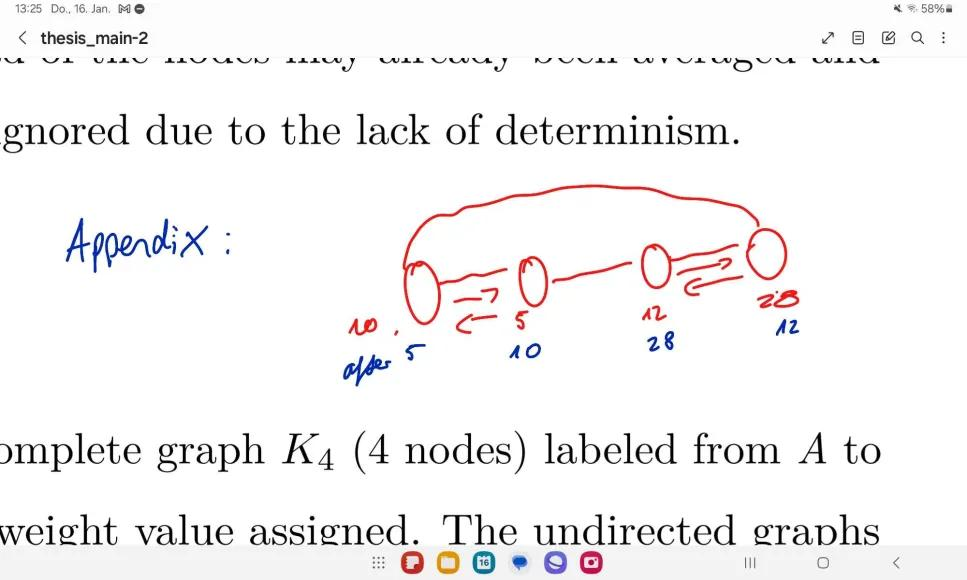
\includegraphics{figures/placeholder/example_ring_problem.jpg}}
    \caption{Example Ring Graph}
    \label{fig:exampleRingProblem}
\end{figure}